\section{Содержание}

\begin{frame}
\begin{center}
\frametitle{Содержание}
\framesubtitle{\ }
\begin{itemize}
\item {\large Введение}
\vspace{0.3cm}
\item {\large Цели работы}
\vspace{0.3cm}
\item {\large Математическая модель трехфазной фильтрации}
\vspace{0.3cm}
\item {\large Алгоритм расчета модели}
\vspace{0.3cm}
\item {\large Параллельная реализация алгоритма}
\vspace{0.3cm}
\item {\large Тестовые задачи}
\vspace{0.3cm}
\item {\large Анализ производительности системы}
\vspace{0.3cm}
\item {\large Заключение}
\end{itemize}
\end{center}
\end{frame}

\section{Введение}

\begin{frame}
\begin{center}
\frametitle{Введение}
\framesubtitle{\ }
\begin{figure}
\begin{minipage}[h]{0.43\textwidth}
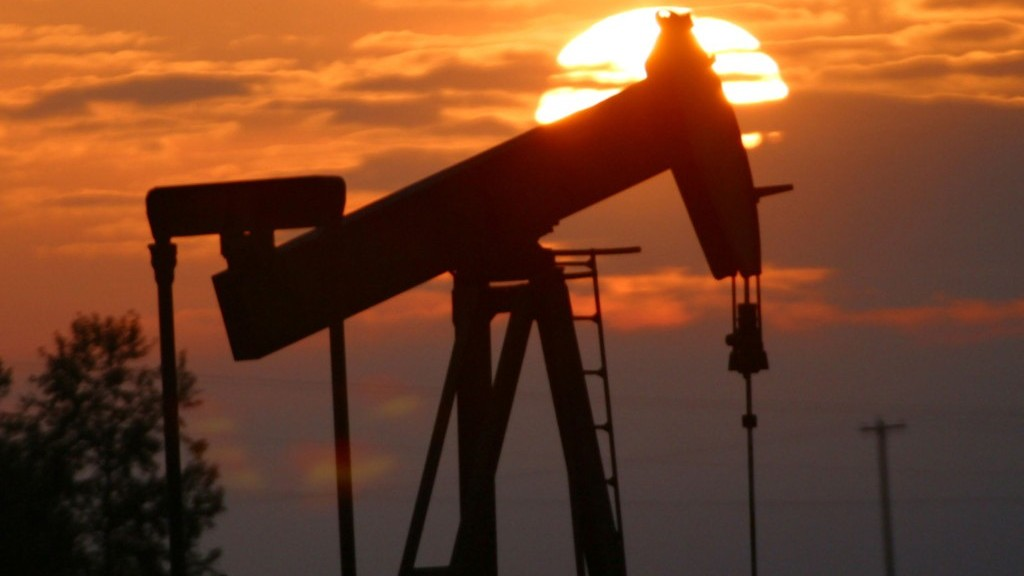
\includegraphics[width=1.0\textwidth]{oil_pump169.jpg}
\caption{\small{Добыча нефти и газа\\ \ }}
\end{minipage}
\hspace{8mm}
\begin{minipage}[h]{0.43\textwidth}
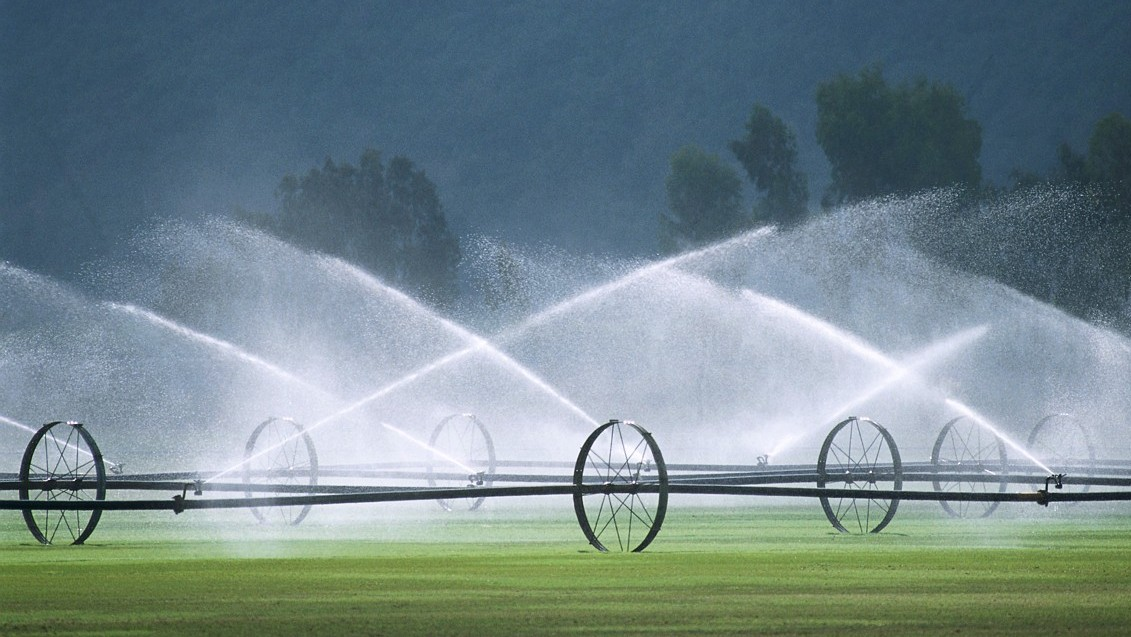
\includegraphics[width=1.0\textwidth]{melio169.jpg}
\caption{\small{Мелиоративные сооружения\\ \ }}
\end{minipage}
\vfill
\begin{minipage}[h]{0.43\textwidth}
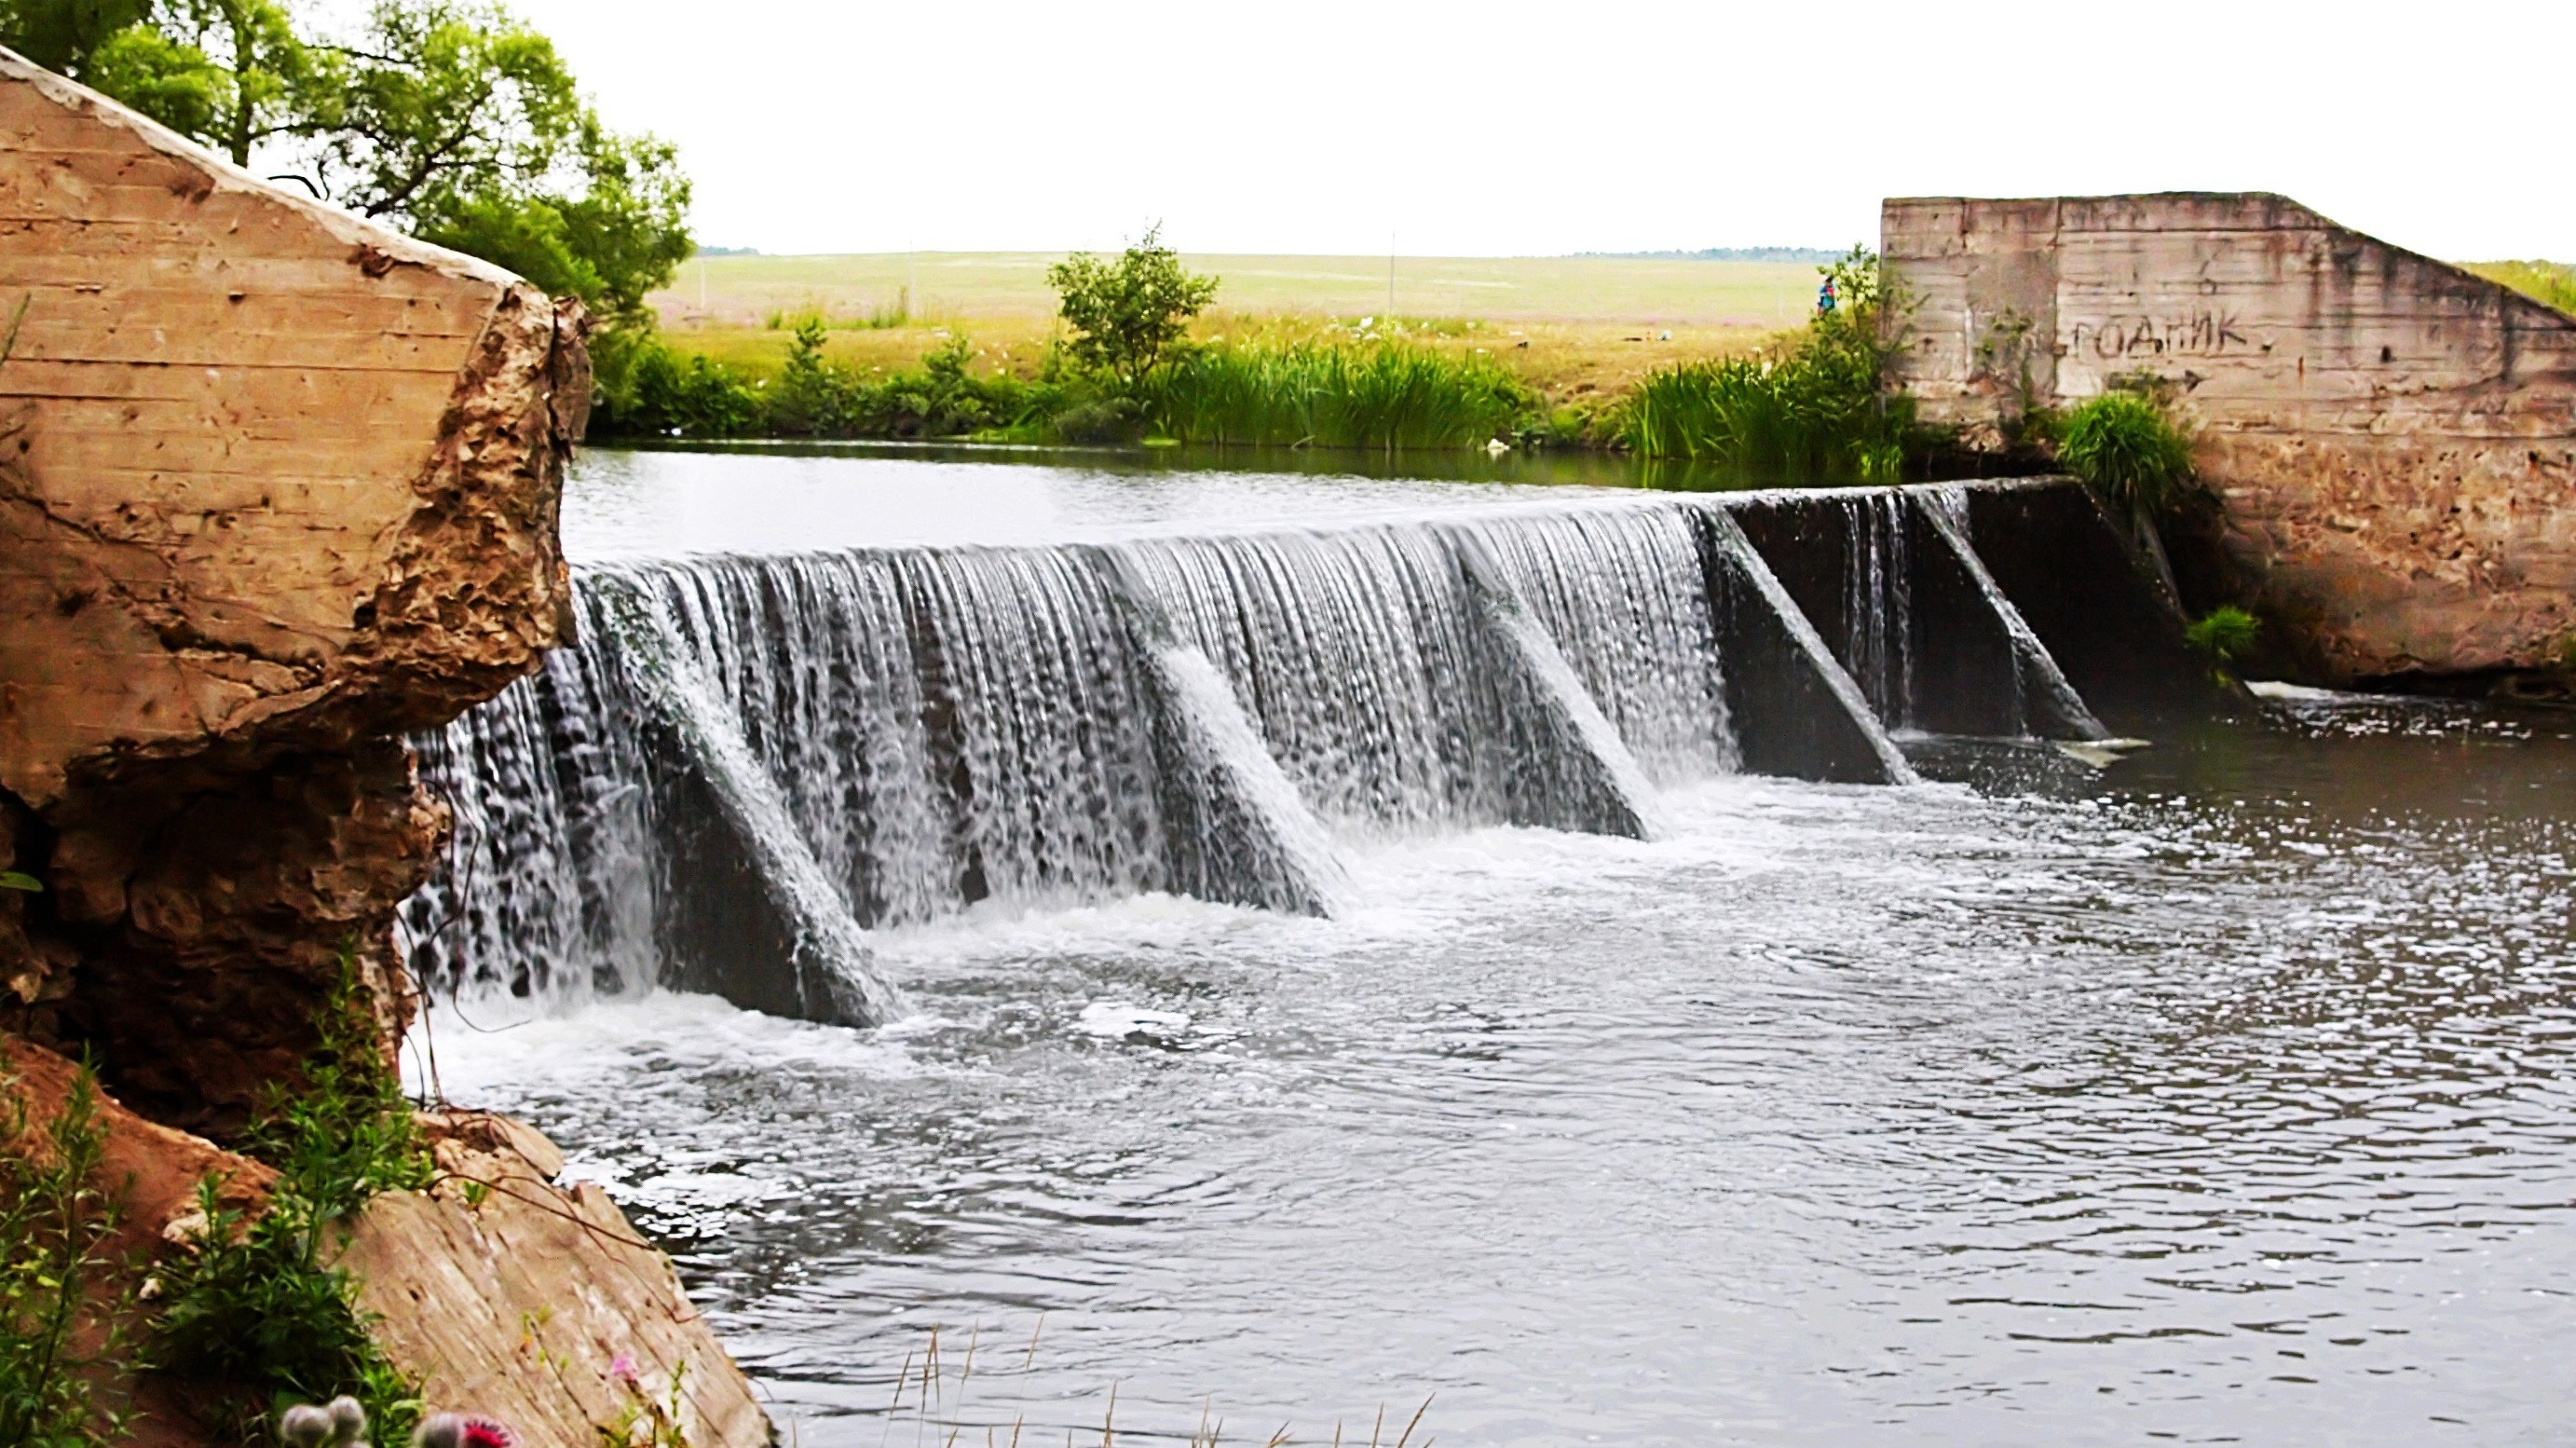
\includegraphics[width=1.0\textwidth]{plotina169.jpg}
\caption{\small{Гидротехнические сооружения}}
\end{minipage}
\hspace{8mm}
\begin{minipage}[h]{0.43\textwidth}
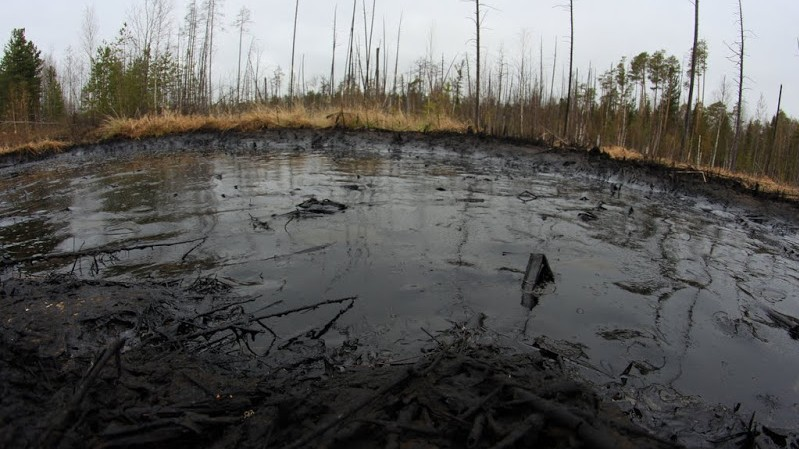
\includegraphics[width=1.0\textwidth]{dirty169.jpg}
\caption{\small{Решение экологических проблем}}
\end{minipage}
\end{figure}
\end{center}
\end{frame}

\section{Цели работы}

\tikzstyle{itembox} = [rectangle, rounded corners, minimum width=1.5cm, minimum height=1.5cm, text centered, draw=black, fill=GreenYellow!50]

\begin{frame}
\begin{center}
\frametitle{Цели работы}
\framesubtitle{\ }
\begin{figure}
  \begin{minipage}[h]{0.2\textwidth}
    
\includegraphics[width=1.0\textwidth]{aim.png}
  \end{minipage}
  \hspace{-1cm}
  \begin{minipage}[h]{0.75\textwidth}
    \begin{tikzpicture}[]
      \node (item1) [itembox, xshift=5.0cm] {Математическая модель};
      \node (item2) [itembox, right of=item1, xshift=4.5cm, yshift=-0.5cm]{Явные численные методы};
      \node (item3) [itembox, below of=item1, xshift=2.0cm, yshift=-1.0cm] {Алгоритм};
      \node (item4) [itembox, below of=item2, yshift=-1.0cm] {Программа};
      \node (item5) [itembox, below of=item3, yshift=-1.0cm] {Многопроцессорные системы};
      \node (item6) [itembox, left of=item5, xshift=-1.0cm, yshift=-2.0cm] {Графические ускорители};
      \node (item7) [itembox, below of=item5, xshift=3.0cm, yshift=-1.0cm] {Тестовые задачи};
    \end{tikzpicture}
  \end{minipage}
\end{figure}
\end{center}
\end{frame}

\section{Математическая модель трехфазной фильтрации}

\begin{frame}
\begin{center}
\frametitle{Математическая модель трехфазной фильтрации}
\framesubtitle{Основные предположения}
\begin{itemize}
\item Трехфазные течения: вода, легкая нефть и газ
\vspace{0.3cm}
\item Фазы несмешивающиеся
\vspace{0.3cm}
\item Жидкости слабосжимаемые
\vspace{0.3cm}
\item Газ идеальный
\vspace{0.3cm}
\item Среда пористая, однородная, изотропная, неподвижная
\vspace{0.3cm}
\item Учитываются капиллярные силы и гравитационное поле
\vspace{0.3cm}
\item Учитываются тепловые процессы
\end{itemize}
\end{center}
\end{frame}

\begin{frame}
\begin{center}
\frametitle{Математическая модель трехфазной фильтрации}
\framesubtitle{Полная система уравнений}
\begin{equation*}
\left\{
  \begin{aligned}
    & \text{1)}\ \frac{\partial \left(m {\sum\limits_{i}{\rho_i S_i E_i(P_i, T)}} + (1-m){\rho_r E_r(P_w, T)}\right)}{\partial t} + \\
    & \qquad + div(\sum_{i}{\rho_i H_i(T) \overrightarrow{u_i}}) = div(\lambda_{eff} grad T),\\
    & \text{2)}\ \frac{\partial (m \rho_i S_i)}{\partial t}+ div(\rho_i \overrightarrow{u_i}) = \rho_i q_i,\\
    & \text{3)}\ \overrightarrow{u_i}=-K \frac{k_i}{{\mu_i(T)}}(grad P_i - {\rho}_i\overrightarrow{g}),\\
    & \text{4)}\ S_w + S_n + S_g=1,\\
    & \text{5)}\ P_n=P_w+P_{cnw}(\overline{S_w}),\quad P_g=P_w+P_{cnw}(\overline{S_w})+P_{cgn}(\overline{S_g}),\\
    & \text{6)}\ k_w=k_w(\overline{S_w}),\quad k_g=k_g(\overline{S_g}),\quad k_n=k_n(\overline{S_w},\overline{S_n}),\\
    & \text{7)}\ \rho_i=\rho_i(P_i,T),\\
    &i=w,n,g. \\
  \end{aligned}
\right.
\end{equation*}
\end{center}
\end{frame}

\begin{frame}
\begin{center}
\frametitle{Математическая модель трехфазной фильтрации}
\framesubtitle{Полная система уравнений с модифицированным уравнением неразрывности}
\begin{equation*}
\left\{
  \begin{aligned}
    & \text{1)}\ \frac{\partial \left(m {\sum\limits_{i}{\rho_i S_i E_i(P_i, T)}} + (1-m){\rho_r E_r(P_w, T)}\right)}{\partial t} + \\
    & \qquad + div(\sum_{i}{\rho_i H_i(T) \overrightarrow{u_i}}) = div(\lambda_{eff} grad T),\\
    & \text{2)}\ \frac{\partial (m \rho_i S_i)}{\partial t}+ div(\rho_i \overrightarrow{u_i}) = \rho_i q_i\textcolor{red}{ + l c_i \cdot div(grad(\rho_i S_i))}, \\
    & \text{3)}\ \overrightarrow{u_i}=-K \frac{k_i}{{\mu_i(T)}}(grad P_i - {\rho}_i\overrightarrow{g}),\\
    & \text{4)}\ S_w + S_n + S_g=1,\\
    & \text{5)}\ P_n=P_w+P_{cnw}(\overline{S_w}),\quad P_g=P_w+P_{cnw}(\overline{S_w})+P_{cgn}(\overline{S_g}),\\
    & \text{6)}\ k_w=k_w(\overline{S_w}),\quad k_g=k_g(\overline{S_g}),\quad k_n=k_n(\overline{S_w},\overline{S_n}),\\
    & \text{7)}\ \rho_i=\rho_i(P_i,T),\\
    &i=w,n,g. \\
  \end{aligned}
\right.
\end{equation*}
\end{center}
\end{frame}